%%%%%%%%%%%%%%%%%%%%%%%%%%%%%%%%%%%%%%%%%%%%%%%%%%%%%%%%%%%%%%%%%%%%%%%%%%%%%%%%%
% Beamer presentationtion 															
% LaTeX Template 																
% Version 1.0 (10/11/12)														%
% This template has been downloaded from: http://www.LaTeXTemplates.com 		%
% https://www.sharelatex.com/blog/2013/08/14/beamer-series-pt2.html
% https://www.writelatex.com/docs?snip_uri=http://www.latextemplates.com/templates/presentations/1/presentation_1.zip				
% License: CC BY-NC-SA 3.0 (http://creativecommons.org/licenses/by-nc-sa/3.0/)  
% Compilar: pdflatex ficheiroTex.tex
%%%%%%%%%%%%%%%%%%%%%%%%%%%%%%%%%%%%%%%%%%%%%%%%%%%%%%%%%%%%%%%%%%%%%%%%%%%%%%%%%

%----------------------------------------------------------------------------------------
%	PACKAGES AND THEMES
%----------------------------------------------------------------------------------------

\documentclass[10pt]{beamer}

\mode<presentation> {

% The Beamer class comes with a number of default slide themes
% which change the colors and layouts of slides. Below this is a list
% of all the themes, uncomment each in turn to see what they look like.

%\usetheme{default}
%\usetheme{AnnArbor}
%\usetheme{Antibes}
%\usetheme{Bergen}
%\usetheme{Berkeley}
%\usetheme{Berlin}
%\usetheme{Boadilla}
%\usetheme{CambridgeUS}
%\usetheme{Copenhagen}
%\usetheme{Darmstadt}
%\usetheme{Dresden}
%\usetheme{Frankfurt}
%\usetheme{Goettingen}
%\usetheme{Hannover} OK
%\usetheme{Ilmenau} OK
%\usetheme{JuanLesPins}
%\usetheme{Luebeck} OK
%\usetheme{Madrid}
%\usetheme{Malmoe}
%\usetheme{Marburg}
%\usetheme{Montpellier}
%\usetheme{PaloAlto}
%\usetheme{Pittsburgh}
%\usetheme{Rochester}
%\usetheme{Singapore}
%\usetheme{Szeged}
\usetheme{Warsaw}
%\usetheme[progressbar=frametitle]{metropolis}
% As well as themes, the Beamer class has a number of color themes
% for any slide theme. Uncomment each of these in turn to see how it
% changes the colors of your current slide theme.

%\usecolortheme{albatross}
%\usecolortheme{beaver}
%\usecolortheme{beetle}
%\usecolortheme{crane}
%\usecolortheme{dolphin}
%\usecolortheme{dove}
%\usecolortheme{fly}
%\usecolortheme{lily}
%\usecolortheme{orchid}
%\usecolortheme{rose}
%\usecolortheme{seagull}
%\usecolortheme{seahorse}
%\usecolortheme{whale}
%\usecolortheme{wolverine}

%\setbeamertemplate{footline} % To remove the footer line in all slides uncomment this line
%\setbeamertemplate{footline}[page number] % To replace the footer line in all slides with a simple slide count uncomment this line

\setbeamertemplate{navigation symbols}{} % To remove the navigation symbols from the bottom of all slides uncomment this line
}
\usepackage{appendixnumberbeamer}
\usepackage{booktabs}
\usepackage[scale=2]{ccicons}
\usepackage{pgfplots}
\usepgfplotslibrary{dateplot}
\usepackage{xspace}
\newcommand{\themename}{\textbf{\textsc{metropolis}}\xspace}
%\usepackage{graphicx} % Allows including images
%\usepackage{booktabs} % Allows the use of \toprule, \midrule and \bottomrule in tables
%\usepackage[utf8]{inputenc} %Permite a utilização dos carateres portugueses
\usepackage{verbatim} %Permite inserir os comentários
%\usepackage{graphicx} %Permite inserir gráficos
%\usepackage[portuguese]{babel} % Para termos texto em português, e.g. legendas e datas
%\usepackage[english]{babel}
%\setbeamertemplate{caption}[numbered] %para numerar os captions
\setbeamertemplate{navigation symbols}{}
%\usepackage[labelfont=scriptsize,labelfont=bf,font=scriptsize,belowskip=-15pt,aboveskip=5pt]{caption}

\title[Dropout Prediction]{Prediction customer dropout using machine learning} 
\subtitle{Current situation} 
% The short title appears at the bottom of every slide, the full title is only on the title page

\begin{comment} % Estrutura da apresentação

Introduction:
Customer analysis is fundamental to develop business and marketing intelligence (Sheth, Mittal, & Newman, 1998), supporting
the understanding of historical data identifying trends and patterns (Berry & Linoff, 2004). The comprehension when
customers dropout, which are the factors related to dropout? What are the patterns¿ related to dropout? Moreover, when this
dropout occurs? Are questions of interest for marketing researchers and business analysts. Information that can be employed to
develop better communications to the customers and appropriate strategies to increase their Customer Lifetime Value. This
thesis addresses state-of-the-art data mining and machine learning technics used to predict dropout and to understand when it
occurred and which factors are related. This insight allows us to propose a a retention system to reduce dropout in customers in
a contractual setting.

Reseach plan:
	1. Developing the systematic literature review supporting the thesis: Dropout Prediction: A Systematic Literature Review
	2. Exploring existing machine learning approaches to predict dropout
	3. Creation of an ensemble method to improve dropout prediction accuracy
	4. Developing article addressing an ensemble method
	5. Finishing and thesis delivery

Methodology:
SLR
For the development of the systematic literature review was adopted, the methodology applied by Kitchenham & Charters (2007) 
developed in three stages: Planning, Implementation Conduct and Results. The planning involves the definition of the research 
need, identification of the research questions and the development of the review protocol. The stage of conducting involves 
research identification, study selections, quality assessment, data extraction, finishing with the data synthesis. 
The last stage develops one activity, report review.

Propose an ensemble of technics to create a voting system for dropout prediction and selecting the most relevant features to anticipate dropout, to support lines of action
that managers and marketing researchers can employ. Allow the identifications of the timmings related to the dropout in a
business context. The employed tasks are according to the business interest are classification; estimation; prediction; affinity
grouping; clustering and description, and profiling. Is also proposed a retention system combining the developed tasks to
increase the Customer Lifetime Value developing a case-study.
Development of a case study using an information system of a Portuguese Software company that provides solution for sport clubs 
using a business model of a software as a service (SaS).


Results:


Explicar o que foi feito...
A análise de dados que vai ser realizada...

Criação de um ensemble method to increase the accuracy to dropout predicting...


\end{comment}

\author[Sobreiro, Berrocal, Alonso]{Pedro Sobreiro, Javier Berrocal (Thesis Supervisor), José Garcia Alonso (Co-supervisor), } % Your name
\institute[UNEX] % Your institution as it will appear on the bottom of every slide, may be shorthand to save space
{ 
University of Extremadura ~~~~~~~~~~~~~~~% Your institution for the title page
\medskip
\textit{pdealexa@alumnos.unex.es} % Your email address
}
\date{Webinar, 11 September 2020} % Date, can be changed to a custom date

\begin{document}

\begin{frame}
	\titlepage % Print the title page as the first slide
\end{frame}

\begin{frame}
\frametitle{Summary} % Table of contents slide, comment this block out to remove it
\tableofcontents % Throughout your presentation, if you choose to use \section{} and \subsection{} commands, these will automatically be printed on this slide as an overview of your presentation

\end{frame}

%----------------------------------------------------------------------------------------
%	PRESENTATION SLIDES
%----------------------------------------------------------------------------------------

%------------------------------------------------
\section{Introduction} % A subsection can be created just before a set of slides with a common theme to further break down your presentation into chunks
%------------------------------------------------
\begin{comment}

\end{comment}

\begin{frame}
	\frametitle{Research goals}
	% Vamos colocar os objetivos do estudo 
	\Large{This thesis focuses in applying machine learning techniques aiming to find answers to the following questions:} \normalsize
	\begin{itemize}
		\item Q1: Which are the patterns related to dropout?
		\item Q2: There are temporal patterns related to the dropout?
		\item Q3: Is possible to increase customer lifetime value employing machine learning techniques? 
	\end{itemize}
	These questions are supported in a Systematic Literature Review, establishing the state of the art in this research area. Our aim is to 
	identify information that can be employed to increase their Customer Lifetime Value, which allows us to develop insights 
	to support retention systems to reduce dropout in customers in a contractual setting.
	
\end{frame}


\begin{comment}
	Reseach plan:
	1. Developing the systematic literature review supporting the thesis: Dropout Prediction: A Systematic Literature Review
	2. Exploring existing machine learning approaches to predict dropout
	3. Creation of an ensemble method to improve dropout prediction accuracy
	4. Developing article addressing an ensemble method using a case study
	5. Finishing and thesis delivery
\end{comment}
\begin{frame}
	\frametitle{Research plan}
	% Vamos colocar os objetivos do estudo 
	\begin{enumerate}
		\item Developing the systematic literature review supporting the thesis: "Dropout Prediction: A Systematic Literature Review" (in progress)
		\item Exploring existing machine learning techniques to predict dropout (in progress)
		\item Creation of an ensemble method to improve dropout prediction accuracy
		\item Developing article addressing an ensemble method using a case study
		\item Finishing and thesis delivery
	\end{enumerate}
\end{frame}

\begin{frame}
	\frametitle{Research plan}
	% Vamos colocar os objetivos do estudo 
	\begin{figure}
		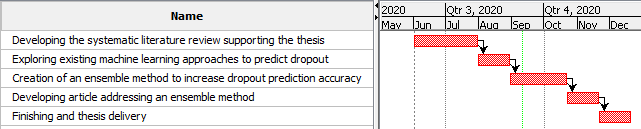
\includegraphics[scale=0.5]{../img/chronogram.png}
		\caption{Activities timeline}
		\label{figure1}
	\end{figure}
\end{frame}

\section{Theoretical background}
\begin{frame}
	\frametitle{Introduction}
	\Large
	\textbf{Some background...}\\
		\begin{itemize} \normalsize
			\item Customer analysis is fundamental to develop business and marketing intelligence \footnotesize(Sheth, Mittal, \& Newman, 1998)\normalsize, supporting the understanding of historical data identifying trends and patterns \footnotesize(Berry \& Linoff, 2004)\normalsize;
			\item This process is also known as data mining, the extraction of knowledge from data \footnotesize(Han \& Kamber, 2006)\normalsize;
			\item According to \footnotesize Han, Kamber, and Pei (2012)\normalsize, these tasks present many similarities between data mining and machine learning;
		\end{itemize}	
	\tiny
	~~~~Sheth, J. N., Mittal, B., \& Newman, B. (1998). Customer Behavior: Consumer Behavior and Beyond (1 edition). Fort Worth, TX: South-Western College Pub. \\
	~~~~Berry, M. J. A., \& Linoff, G. (2004). Data mining techniques: For marketing, sales, and customer relationship management (2nd ed). Indianapolis, Ind: Wiley Pub.\\
	~~~~Han, J., \& Kamber, M. (2006). Data mining: Concepts and techniques (2nd ed). Amsterdam; Boston: San Francisco, CA: Elsevier; Morgan Kaufmann.\\
	~~~~Han, J., Kamber, M., \& Pei, J. (2012). Data mining: Concepts and techniques (3. ed). Amsterdam: Elsevier; Morgan Kaufmann.\\

\end{frame}

\begin{frame}
	\frametitle{Introduction}
	\Large
	\textbf{Some background...}\\
		\begin{itemize} \normalsize
			\item Machine learning could be used to extract knowledge to understand dropout for the development of effective retention strategies \footnotesize(Verbeke, Martens, Mues, \& Baesens, 2011)\normalsize;
			\item Machine learning algorithms have been used to predict customer dropout \footnotesize(Bandara, Perera, \& Alahakoon, 2013)\normalsize, without however to consider the timings of the dropout;
			\item Machine learning can be used to develop of customer retention strategies based on existing data \footnotesize(Verbeke et al., 2011)\normalsize, extracting patterns from data \footnotesize(Kelleher et al., 2015)\normalsize, that support the development of counteractions before an event occurs.
		\end{itemize}	
	\tiny
	~~~~Verbeke, W., Martens, D., Mues, C., \& Baesens, B. (2011). Building comprehensible customer churn prediction models with advanced rule induction techniques. Expert Systems with Applications, 38(3), 2354–2364. doi: 10.1016/j.eswa.2010.08.023 \\
	~~~~Bandara, W. M. C., Perera, A. S., \& Alahakoon, D. (2013). Churn prediction methodologies in the telecommunications sector: A survey. 2013 International Conference on Advances in ICT for Emerging Regions (ICTer), 172–176. doi: 10/ggtgjg\\
	~~~~Verbeke, W., Martens, D., Mues, C., \& Baesens, B. (2011). Building comprehensible customer churn prediction models with advanced rule induction techniques. Expert Systems with Applications, 38(3), 2354–2364. doi: 10.1016/j.eswa.2010.08.023\\
\end{frame}

\begin{frame}
	\frametitle{Introduction}
	\Large
	\textbf{Some background...}\\
		\begin{itemize} \normalsize
			\item The identification of the dropout can be developed in different contexts: customers that buy in contractual settings and non-contractual settings where a firm have to infer if the customer is still active \footnotesize(Gupta et al. ,2006) \normalsize;
			\item The main characteristic of a contractual setting is a contact of the customer canceling a subscription \footnotesize(Fader \& Hardie, 2007)\normalsize;
			\item Customer dropout prediction should consider the context, where there is a contractual or non-contractual setting.
		\end{itemize}	
	\tiny
	~~~~Gupta, S., Hanssens, D., Hardie, B., Kahn, W., Kumar, V., Lin, N., … Sriram, S. (2006). Modeling Customer Lifetime Value. Journal of Service Research, 9(2), 139–155. doi: 10.1177/1094670506293810 \\
	~~~~Fader, P. S., \& Hardie, B. G. S. (2007). How to project customer retention. Journal of Interactive Marketing, 21(1), 76–90. doi: 10.1002/dir.20074\\
\end{frame}
\begin{comment}
customers that buy in contractual settings, for example cellular phones, magazines subscriptions where is an inform by the customer ending the relation and non-contractual settings for example buying a book from amazon, where a firm have to infer if the customer is still active 
\end{comment}

\begin{frame}
	\frametitle{Introduction}
	\Large
	\textbf{Summary}\\
		\begin{itemize} \normalsize

			\item It is also know, that the costs of retaining customers are lower when compared to the costs of attracting new ones \footnotesize(Edward \& Sahadev, 2011)\normalsize, reinforced by that the reduction of the dropout rates could represent an increase in the profits \footnotesize(Reichheld, 1996)\normalsize;
			\item Machine learning algorithms have been used to predict customer dropout \footnotesize(Bandara, Perera, \& Alahakoon, 2013)\normalsize;
			\item But, to our knowledge, there is a lack of an overview of research related to the use of machine learning techniques to target customer dropout with contractual settings considering also the timings of the dropout.
			
		\end{itemize}	
	\tiny
	~~~~Edward, M., \& Sahadev, S. (2011). Role of switching costs in the service quality, perceived value, customer satisfaction and customer retention linkage. Asia Pacific Journal of Marketing and Logistics, 23(3), 327–345. doi: 10.1108/13555851111143240 \\
	~~~~Reichheld, F. F. (1996, Março 1). Learning from Customer Defections. Harvard Business Review, (March–April 1996). Retrieved from https://hbr.org/1996/03/learning-from-customer-defections \\
	~~~~Bandara, W. M. C., Perera, A. S., \& Alahakoon, D. (2013). Churn prediction methodologies in the telecommunications sector: A survey. 2013 International Conference on Advances in ICT for Emerging Regions (ICTer), 172–176. doi: 10/ggtgjg\\
\end{frame}

\begin{frame}
	\frametitle{Research gap}
	% Vamos colocar os objetivos do estudo 
	\textbf{\large{Considering this context, this research tries to analyze the state of the art to identify Machine Learning studies to predict customer dropout to support the development of counteractions before the customer churns, considering also when it occurs.}}
\end{frame}

\section{Methodology}
\begin{comment}
Dropout predicting is challenging analysis process which requires appropriate approaches to address the dropout. Existing approaches are applied in different areas such as education, telecommunications, retail, social networks, and banking services. The goal is to identify customers in the risk of dropout to support retention strategies. This research developed a systematic literature review to evaluate the development of existing studies to predict dropout using machine learning,  following the guidelines recommended by Kitchenham and Peterson. The systematic review followed three phases planning, conducting and reporting. The selection of the most relevant articles was based on the use of Active Systematic Review tool using artificial intelligence algorithms. The criteria identified 28 articles and several research lines where identified. Dropout is a transversal problem for several sectors of economic activity, where it can be taken countermeasures before it happens if detected early.	
\end{comment}
\begin{frame}
	\frametitle{Methodology}
	\begin{itemize}
		\item Was developed a Systematic Literature Review (SLR) in three stages \footnotesize(Kitchenham \& Charters, 2007)\normalsize: Plan, Conduct and Report;
		\item Plan: definition of the research need, identification of the research questions and the development of the review protocol;
		\item Conduct: research identification, study selections, quality assessment, data extraction, finishing with the data synthesis;
		\item Report: stage that develops the activity report review.
	\end{itemize}
	\tiny 
	~~~~Kitchenham, B., \& Charters, S. (2007). Guidelines for performing structural literature reviews in software engineering (pp. 1–26) [Joint technical report]. Australia: Keele Univ., and Empirical Software Eng., Nat’l ICT.\\
\end{frame}
\begin{comment}

\end{comment}

\begin{frame}
	\frametitle{Systematic Literature Review Phases}
	\begin{figure}
		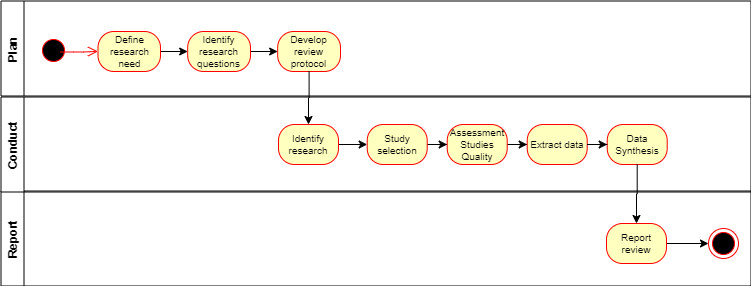
\includegraphics[scale=0.5]{../img/slr_phases.png}
		\caption{SLR phases based on Kitchenham and Charter (2007)}
		\label{figure1}
	\end{figure}
\end{frame}

\begin{frame}
	\frametitle{Research questions}
	What is the current state of machine learning research in existing studies to predict dropout in contractual settings? Based in this question were identified the following questions:
	\begin{itemize}
		\item RQ1: What studies have been published?;
		\item RQ2: Which algorithms have been used to predict the dropout? This question will also address algorithms used by business area (as suggested in activity 6)
		\item RQ3: What are the more relevant features related to predicting customer dropout?
		\item RQ4: When the dropout occurs? 
		\item RQ5: What is the accuracy of the machine learning algorithms to predict dropout?
	\end{itemize}
\end{frame}
\begin{comment}
RQ1: aims to identify what researches have been published so far in the area. This will allow to understand the extent of the research being developed. 
RQ2: aim to identify which different types of machine learning algorithms used to predict the dropout (RQ2) to deep the knowledge of the approaches being used to address the dropout. 
RQ3: explores which features are being used to predict the dropout. 
RQ4: Intends to understand if the timing related to the customer dropout is considered, this question explores if any study explores the advantage of using survival analysis, considering that allows also to examine if an event occurs but also how long took to occur (Williams, 2008). This perspective entails the understanding if is also covered the timings of the dropout event in the potential research to be explored. 
RQ5: aims to identify the accuracy of machine learning algorithms to predict the dropout. The goal of the prediction in the dropout is to develop classification task,  according to Rätsch (2004) is to find a functional mapping between the input data X, describing the input pattern, to a class label Y, such that Y=f(X), where the aim is to accurately predict the correct label on unseen data. However should be used appropriate performance measures, e.g. if the data is imbalanced should be considered the use of accuracy (Chawla, Bowyer, Hall, & Kegelmeyer, 2002)
\end{comment}

\begin{frame}
	\frametitle{Population, Intervention, Comparison, Outcomes and Context}
\begin{center}
\begin{table}
  \centering
  \scriptsize
  \caption{
  	PICOC criteria
  	}
    \begin{tabular}{p{3cm} p{5cm}}
    \toprule
    PICOC & Description\\
    \midrule
	Population & Research papers about dropout with contractual settings \\ \hline
	Intervention &  Machine learning algorithms to predict dropout	\\ \hline	
	Comparison & Studies addressing machine learning algorithms to predict dropout \\ \hline 
	Outcome & Synthesis identifying research questions, gaps in the research domain and also best practices identified \\ \hline
	Context & Academia and industry\\
\bottomrule
\end{tabular}
\label{Abordagens analisadas}
\begin{flushleft}
	Note: Context (PICOC) as suggested Kitchenham and Charters (2007) and proposed by Petticrew and Roberts (Petticrew \& Roberts, 2006) to support the development of the search string.
\end{flushleft}
\end{table}
\end{center}
	\tiny 
~~~~Kitchenham, B., \& Charters, S. (2007). Guidelines for performing structural literature reviews in software engineering (pp. 1–26) [Joint technical report]. Australia: Keele Univ., and Empirical Software Eng., Nat l ICT.\\
~~~~Petticrew, M., \& Roberts, H. (2006). Systematic reviews in the social sciences: A practical guide. Malden, MA ; Oxford: Blackwell Pub.\\
\end{frame}

\begin{frame}
	\frametitle{Search }
	\begin{itemize}
		\item Search string: ((“customer dropout”) OR (“customer churn”) AND “machine learning” AND (“contractual” OR “membership”));
		\item Applied to the title, abstract, and keywords in the search period between January 2000 and June 2020
		\item The exclusion criteria were Books, Non-English articles, patents, and thesis
		\item Sources SpringerLink, Scopus, Science@Direct, ISI Web of Science, IEEE Digital Library, and ACM Digital Library
		\item The selection process was developed using ASReview (ASReview Core Development Team, 2019) creating a dataset of the identified articles, providing five relevant papers and five irrelevant papers to train Machine Learning model Naïve Bayes;
		\\~\\
	\end{itemize}
		\tiny 
~~~~Kitchenham, B., \& Charters, S. (2007). Guidelines for performing structural literature reviews in software engineering (pp. 1–26) [Joint technical report]. Australia: Keele Univ., and Empirical Software Eng., Nat l ICT.\\
~~~~Petticrew, M., \& Roberts, H. (2006). Systematic reviews in the social sciences: A practical guide. Malden, MA ; Oxford: Blackwell Pub.\\
\end{frame}


\section{Results}
\begin{comment} 

\end{comment}

\begin{frame}[fragile]{Results}
  	\begin{itemize}
		\item 449 studies were found: Scopus 210; IEEE 20; SpringerLink	79; Science Direct 126; ISI Web of Knowledge 6 and ACM 8
) in the first step of the conduct (Identify research);
		\item 20 incomplete items were removed
		\item 16 duplicates were removed
		\item 335 were removed after ASReview
		\item 78 papers selected
		\item Data analysis procedure available \href{https://github.com/pesobreiro/dropoutPredFitness}{\color{red}{here}}.
	\end{itemize}
\end{frame}
\begin{comment}
	1.	Selected randomly some articles and are identified as relevant and irrelevant, at least 5 each. ASReview suggests when to stop;
	2.	ASReview orders the publications in such a way that you see the most relevant publications first
	3.	Stopping criterium could be stopping after n presented abstracts were labeled irrelevant, or if your time is up. You can use the chart in the statistics panel to follow your progress" 
\end{comment}

\begin{frame}[fragile]{Results}
	\frametitle{RQ1. What studies have been published?}
	\begin{figure}
		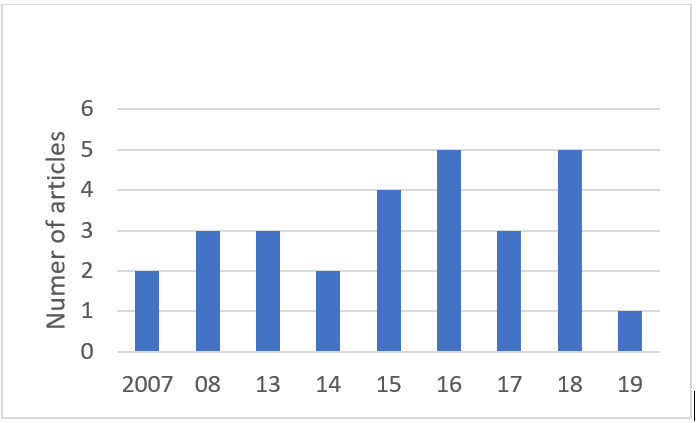
\includegraphics[scale=0.5]{../img/articles_by_Year.png}
		\caption{Articles per year after quality assessment}
		\label{figure2}
	\end{figure}
\end{frame}

\begin{frame}[fragile]{Results}
	\frametitle{RQ1. What studies have been published?}
	\begin{figure}
		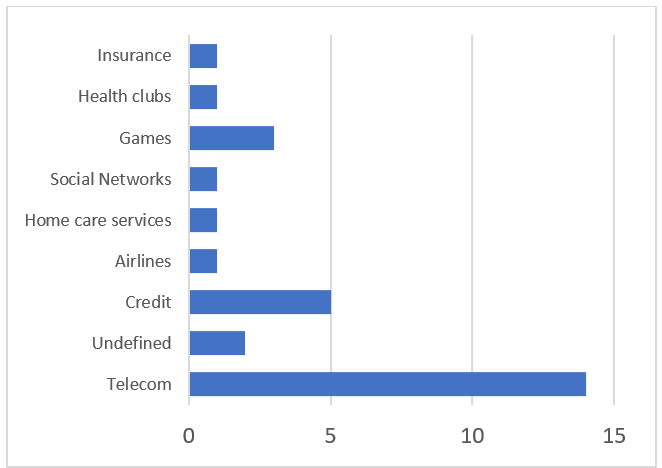
\includegraphics[scale=0.5]{../img/studiesByBusiness.png}
		\caption{The number of studies per business context}
		\label{figure3}
	\end{figure}
\end{frame}

\begin{frame}[fragile]{Results}
	\frametitle{RQ2: Which algorithms have been used to predict the dropout?}
	\begin{figure}
		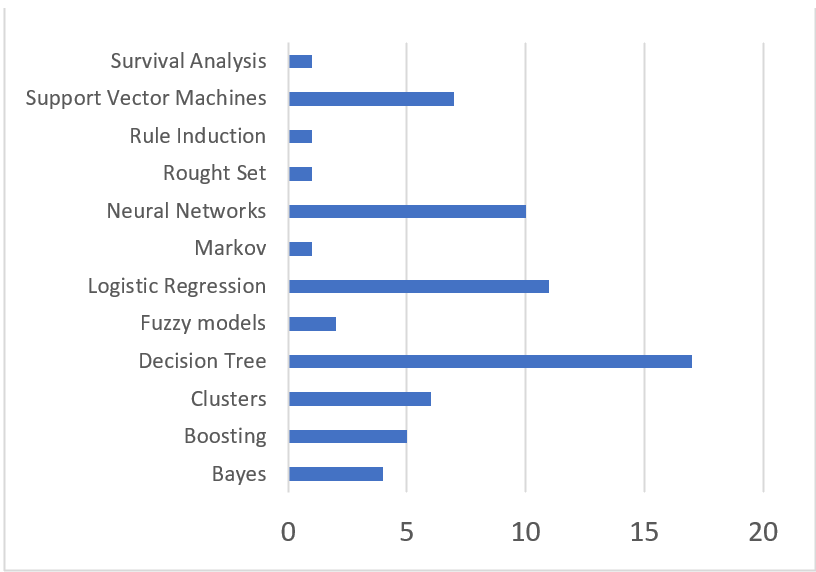
\includegraphics[scale=0.5]{../img/mainAlgorithms.png}
		\caption{Main algorithms used in the analyzed papers}
		\label{figure3}
	\end{figure}
\end{frame}

\begin{frame}[fragile]{Results}
	\frametitle{RQ3: What are the more relevant features related to predicting customer dropout?}
	\begin{figure}
		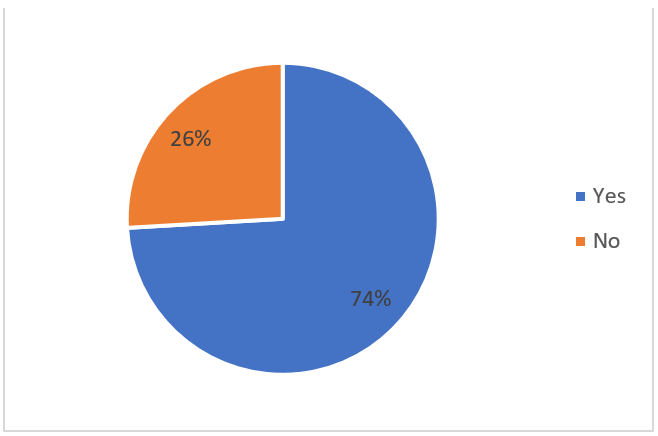
\includegraphics[scale=0.5]{../img/relevantFeatures.png}
		\caption{Percentage of studies identifying the relevant features}
		\label{figure4}
	\end{figure}
\end{frame}
\begin{comment}
	We only retrieved the information if the studies address the features but we need clarify better which are the best predictors
\end{comment}


\begin{frame}[fragile]{Results}
	\frametitle{RQ4: When the dropout occurs?}
	\begin{figure}
		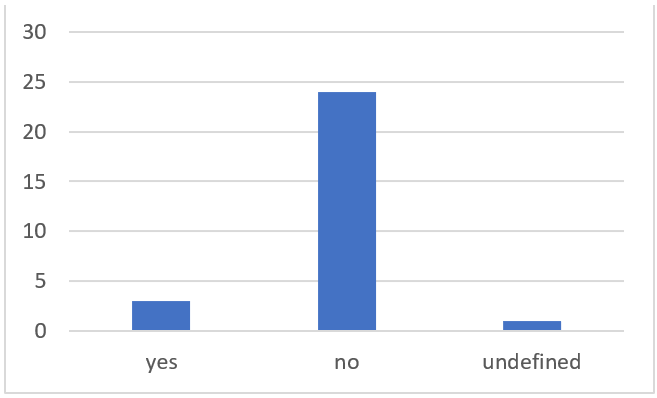
\includegraphics[scale=0.5]{../img/dropoutTimings.png}
		\caption{The number of studies addressing the dropout timings}
		\label{figure4}
	\end{figure}
\end{frame}

\begin{frame}[fragile]{Results}
	\frametitle{RQ5: What is the accuracy of the machine learning algorithms to predict dropout?}
	\begin{figure}
		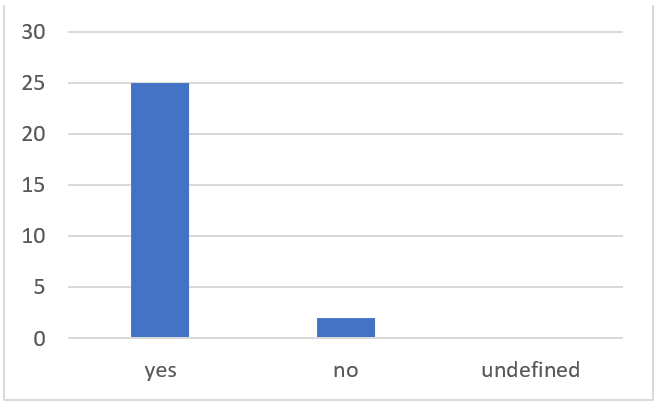
\includegraphics[scale=0.5]{../img/predictionAccuracy.png}
		\caption{Number of studies identifying the prediction accuracy}
		\label{figure3}
	\end{figure}
\end{frame}
\begin{comment}
	We only retrieved the information if the studies address the accuracy but we need to improve exploring the accuracy of existing studies... however this requires a deeper understanting about the quality of the data, imbalanced datasets and how to measure the performance considering the limitations of the accuracy 
\end{comment}

\section{Work in progress}
\begin{frame}
	\frametitle{Exploring existing machine learning techniques}
	\begin{itemize}
		\item Was tested class train/test stratification in the target variable, imbalance datasets, grid search optimization targeting AUC for classification (dropout,non-dropout)
		\item The class imbalance aproaches to adjust the weights inversely proportional to class frequencies in the input data using the library scikit-learn (Pedregosa et al., 2011). 
		\item Hyperparameters optimisation developed using grid search targeting AUC as the optimization goal considering the discriminatory power (Emeterio et al., 2016). 
		\item Logistic Regression (LR), Decision Tree Classifier (DTC), Random Forest Classifier (RFC), and Gradient Boosting Classifier (GBC) best performances in GBC (accuracy, sensitivity, precision, F1 Score) and RFC in AUC.
		\item Code book, dataset and Jupyter notebook \href{https://github.com/pesobreiro/dropoutPredFitness}{\color{red}{code}}
	\end{itemize}
\end{frame}
\begin{comment}
	1.	Sensitivity (SN): True positive rate = TP/(TP+FN) 
	2.	Specificity (SP): True negative rate = TN/(TN+FP)
	3.	Precision: True predicted ‘no dropouts’ against all predicted ‘no dropouts’ true or not TP/(TP+FP)
	4.	F1-Score: Combines precision and sensitivity representing their harmonic mean 2×TP/ (2×TP + FP + FN)
	5.	Receiver Operating Characteristic (ROC) Curve: Representing the model capability to distinguish dropout and non-dropout. Higher AUC (Area Under The Curve) better model prediction 0 and 1;.
\end{comment}
\begin{frame}[fragile]{Results}
	\frametitle{Exploring existing machine learning techniques}
	\begin{figure}
		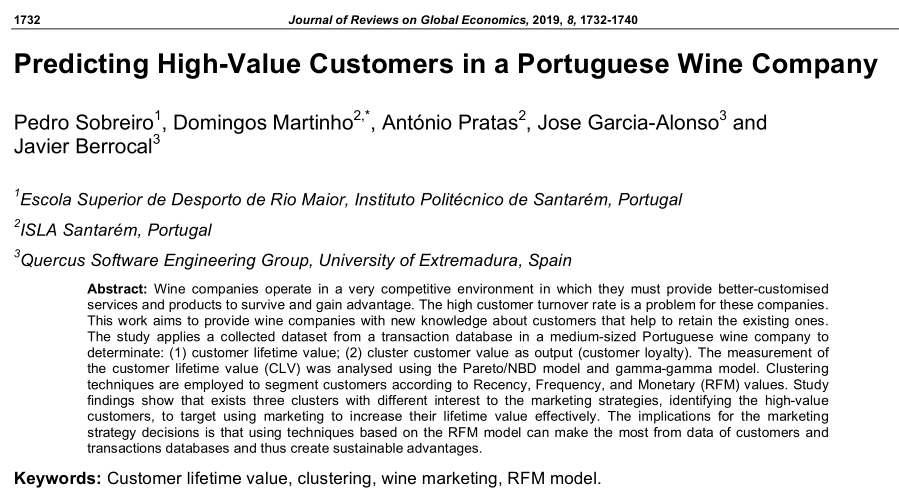
\includegraphics[scale=0.4]{../img/pub1.png}
		\caption{Publication using an technique for Q3 "Is possible to increase customer lifetime value employing machine learning techniques?"}
		\label{figure3}
	\end{figure}
\end{frame}


\section{Conclusion}
\begin{frame}
	\frametitle{Conclusion}
	\begin{itemize}
 		\item The telecommunications sector is the area where are being developed most of the studies, which identifies some research areas gaps that need to be addressed;
 		\item Algorithms to predict dropout using also survival analysis approaches is an area under researched, only three research papers, however  considering the number of citations these approaches getting the attention (Perianez et al., 2016);
 		\item The use of algorithms to explore the timings when the dropout will occur is an approach that could complement the dropout prediction, supporting the development of actions considering both the probability and when should be developed countermeasures to avoid the customer dropout
	\end{itemize}
	\tiny 
	~~~~Perianez, A., Saas, A., Guitart, A., \& Magne, C. (2016). Churn Prediction in Mobile Social Games: Towards a Complete Assessment Using Survival Ensembles. 2016 IEEE International Conference on Data Science and Advanced Analytics (DSAA), 564–573. doi: 10/ggtgjh

\end{frame}


\begin{frame}
\frametitle{}
\normalsize
	\Huge Thanks! \\~\\
	\Large Start where you are. Use what you have. Do what you can. \textbf{Arthur Ashe}
\end{frame}


\end{document}\grid
